\documentclass[
  10pt
, handout
]{beamer}

\usepackage{pgfpages}

% Use T1 Font encoding to support more glyphs
\usepackage[T1]{fontenc}

%\setbeameroption{show notes on second screen}

% Number sections in table of contents
\setbeamertemplate{section in toc}[sections numbered]
% Hide subsections in table of contents
\setcounter{tocdepth}{1}

% Use metropolis beamer theme
\usetheme[
  numbering=fraction  % Page numbering like 3/10
]{metropolis}
\usepackage{appendixnumberbeamer}

\usepackage{booktabs}
\usepackage[scale=2]{ccicons}

\usepackage{pgfplots}
\usepgfplotslibrary{dateplot}

\usepackage{xspace}
\newcommand{\themename}{\textbf{\textsc{metropolis}}\xspace}

\usepackage{graphicx}
\usepackage{listings}

\usepackage{lmodern}

\usepackage{eurosym}
\usepackage{amsmath, amssymb}
\usepackage[binary-units=true]{siunitx}
\DeclareSIUnit{\EUR}{\text{\euro}}

\usepackage{xcolor}
\newcommand\crule[3][black]{\textcolor{#1}{\rule{#2}{#3}}}
\definecolor{aswe-reactive}{cmyk}{1,0.9,0,0}
\definecolor{aswe-proactive}{cmyk}{0.6,0.9,0,0}
\definecolor{aswe-preferences}{cmyk}{0,0.75,1,0}
\definecolor{aswe-data}{cmyk}{0.85,0.1,1,0}

% Content

\title{Voice Controlled User-Interface}
\subtitle{}
\date{April 11, 2019}
\author{Dorian Czichotzki, David Marchi, Daniel Schäfer}

\begin{document}

\maketitle

\begin{frame}{Agenda}
  \tableofcontents[pausesections]
\end{frame}

\section{How does speech recognition work?}  % Dorian

\begin{frame}{General purpose speech recognition}
  \begin{itemize}
      \item Hidden Markov Model transforms spectral information into observations
      \item Observations can be mapped to phoneme or words \\
        $\rightarrow$ 44 phoneme in English language
      \item Words are build up of a sequence of phoneme
  \end{itemize}
\end{frame}

\begin{frame}{Deep recurrent neural networks}
  \begin{itemize}
      \item Large vocabulary speech recognition \\
        $\rightarrow$ English language has more than 1mio. words
        \item Uses raw wave data to analyze time sequences
        \item Results in higher accuracy
  \end{itemize}
\end{frame}

\begin{frame}{End-to-End automatic speech recognition}
    \begin{itemize}
        \item Usually offered as a service due to high compute demand
        \item Employs language and pronunciation models to reason about input
        \item Future: Attention based models learn pronunciation and language models
    \end{itemize}
\end{frame}

\section{Suited Applications and Requirements}  % Dorian

\begin{frame}{What applications are suited for voice control}
  \begin{itemize}
    \item Personal voice assistant
    \item In-car systems \\
        $\rightarrow$ Navigation or telephone controls
    \item Telephony automation \\
        $\rightarrow$ Call center support
    \item People with disabilities \\
        $\rightarrow$ Deaf telephony
  \end{itemize}
\end{frame}

\begin{frame}{Which requirements make voice control necessary?}
  \begin{itemize}
    \item Other means of control are not available
    \item Users attention is needed for other systems \\
        $\rightarrow$ e.g. Fighter jets
  \end{itemize}
\end{frame}

\section{Advantages and disadvantages}  % Daniel

\begin{frame}{Voice controlled dialogs - Advantages}
  Advantages

  \begin{itemize}
    \item<1-> Hands free, eyes free
    \item<2-> No complex menu interaction
    \item<3-> Quick fire and forget command
    \item<4-> Could be capable of asking questions
  \end{itemize}
  \note[item]<2>{Like commandline but for voice}
\end{frame}

\begin{frame}{Speech controlled dialogs - Disadvantages}
  Disadvantages

  \begin{itemize}
    \item<+-> Hard/impossible to enter non-word content
    \item<+-> Low accuracy $\rightarrow$ High chance of not doing what you want
    \item<+-> Often limited to a few predefined actions
    \item<+-> Often robotic, unnatural commands necessary
  \end{itemize}
\end{frame}

\begin{frame}{Speech controlled dialogs - No visuals}
  No visuals

  \begin{itemize}
    \item Doesn't convey information unless it's talking right at this moment
    \item Can't show multiple things at the same time
    \item Is slower because you can't skip anything
    \item If you missed something, you missed it
  \end{itemize}
\end{frame}

\section{Existing Guidelines}  % Daniel

\begin{frame}{Guidelines - Laws}
  \begin{itemize}
    \item[{[.]}] Law of proximity
    \item[{[ ]}] Law of equality
    \item[{[ ]}] Law of closedness
    \item[{[ ]}] Law of continuity
  \end{itemize}
  \note[item]{Objects closer together appear as a single unit}
  \note[item]{Similar objects appear as a group}
  \note[item]{Closed structures are more recognizeable}
  \note[item]{Objects in a line or curve appear as single figure}
\end{frame}

\begin{frame}{Guidelines - Laws}
  \begin{itemize}
    \item[{[x]}]<1-> Law of experience
    \item[{[x]}]<2-> Law of same fate
    \item[{[.]}]<3-> Law of symmetry
    \item[{[x]}]<4-> Law of simplicity
  \end{itemize}
  \note[item]<2->{Objects moving in the same way appear as a group}
  \note[item]<3->{Objects that are arranged in symmetry are more easily recognizable}
  \note[item]<4->{The brain simplifies complex shapes}
\end{frame}

\begin{frame}{Guidelines}
  \begin{itemize}
    \item<+-> Nicht mehr als 3 Infos länger als 7s merken lassen \\
              $\rightarrow$  Nicht zu lange Antworten
    \item<+-> Ablenkung minimieren \\ $\rightarrow$ Nur wichtiges sagen (keine Zeitverschwendung)
    \item<+-> Langsame Antwortzeiten vermeiden
    \item<+-> Fortschrittsanzeigen nutzen \\ $\rightarrow$ Bsp. Alexa blinkender Ring, wenn sie "nachdenkt"
    \item<+-> Varianten zur Erledigung einer Aufgabe minimieren \\ $\rightarrow$ Anti-Guideline bei Sprache
  \end{itemize}
   \note[item]{Möglichst viele Wege, da nicht offensichtlich sieht}
\end{frame}

\begin{frame}{Shneidermans 8 goldene Regeln (1-4)}
  \begin{enumerate}
    \item<+-> Versuche Konsistenz zu erreichen \\
              $\rightarrow$ Gleiche Sprachanfragen, gleiche Aktionen
    \item<+-> Biete erfahrenen Benutzern Abkürzungen an \\
              $\rightarrow$ Eigene Befehle
    \item<+-> Biete informatives Feedback \\
              $\rightarrow$ Ring, "Did you mean?"
    \item<+-> Dialoge sollten abgeschlossen sein \\
              $\rightarrow$ TODO
  \end{enumerate}
\end{frame}

\begin{frame}{Shneidermans 8 goldene Regeln (5-8)}
  \begin{enumerate}
    \setcounter{enumi}{4}
    \item<+-> Biete einfache Fehlerbehandlung \\
              $\rightarrow$ z.b. Kaufbestätigung
    \item<+-> Biete einfache Rücksetzmöglichkeiten (undo) \\
              $\rightarrow$ "Stop!"
    \item<+-> Unterstütze benutzergesteuerten Dialog \\
              $\rightarrow$ Flexibler Dialog
    \item<+-> Reduziere die Belastung des Kurzzeitgedächtnisses \\
              $\rightarrow$ Kurze Antworten
  \end{enumerate}
\end{frame}

\section{Additional Guidelines}  % David

\begin{frame}{Additional Guidelines}
 \begin{enumerate}
  \item<+-> {language very complex} \\
            $\rightarrow$ coping mechanisms

  \item<+-> {accomodate naturale language feeling}
  \item<+-> {make use of benefit}

  \item<+-> {keep scope small}
 \end{enumerate}
\end{frame}


\begin{frame}{Additional Guidelines - 7. Steps Norman}
  \begin{center}
    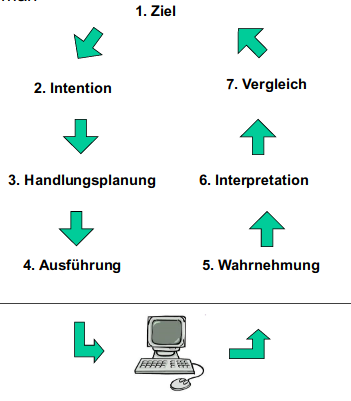
\includegraphics[scale=0.8]{resources/7_steps_norman.png}
  \end{center}
\end{frame}





\section{App Dependent Guidelines}  % David

\begin{frame}{How are the guidelines dependent on the app?}
  \begin{enumerate}
    \item<+-> {degree of user} \\
               $\rightarrow$ beginner, advanced
    \item<+-> {enviroment and context} \\
               $\rightarrow$ special trained speech recognition             
    \item<+-> {integrate with other interactive systems} \\
               $\rightarrow$ more powefull \\         
               $\rightarrow$ visual clues
  \end{enumerate}
\end{frame}

\end{document}
